\documentclass[11pt,a4paper]{article}
\usepackage{fullpage}	% Bigger pages
\usepackage{cite} 		% Include citations
\usepackage{hyperref} 	% Hyperlinks everywhere!
\usepackage{natbib}		% Include bibliography
\usepackage{graphicx}	% Include pictures
\usepackage{amsmath}	% Use \eqref

\begin{document}

\title{Constraining the Hemispherical Structure in the Hidden Layer At the Top of the Earth's Inner Core}
\author{Candidate Number: \\  \\ Supervisor: Prof. Keith Priestley}
\maketitle

\begin{abstract}
Since its discovery in 1936, the Earth's inner core has been well documented by both body wave and normal mode studies. However, one area where properties are not yet well measured is the top of the inner core. The upper region of the inner core is of particular interest as it is thought that as the outer core freezes onto the inner core the variable environment at this boundary is encoded in the properties of the frozen material. 
\end{abstract}

\tableofcontents

\newpage
\section{Introduction}
The inner core was first discovered by Inge Lehmann in 1936, who used the existence of P wave arrivals within the P wave shadow zone to infer a solid-liquid boundary lying within the core mantle boundary (\cite{Lehmann}). Over the following 80 years large progress has been made on measuring the properties of the inner core, but there is much still to learn.

Of particular interest is the velocity and attenuation structure, which can be used to infer the chemical and physical properties of the inner core's constituent material. The following gives a summary of these properties, and is quoted directly from \cite{Deuss2014}:
\begin{itemize}
	\item The top 60-80 km of the inner core is isotropic, and the deeper parts have 3-4\% anisotropy. The anisotropy exists in both velocity and attenuation; waves traveling in the polar direction are faster and more attenuated than waves traveling equatorially.
	\item There may be an innermost inner core with different anisotropy, though evidence is not compelling.\footnote{Research published since \cite{Deuss2014} provides strong evidence for this (\cite{Wang2015}).}
	\item The inner core displays a hemispherical variation: The western hemisphere is more strongly anisotropic, has a lower isotropic compressional velocity, and is less attenuating than the eastern hemisphere. There are sharp boundaries between the two hemispheres.
	\item Inner core superrotation is less than $0.5^{\circ}$ /yr and may even be as small as $0.1-1^{\circ}$ /Myr.
\end{itemize}

The upper inner core is of particular interest, as material from the outer core is currently freezing onto it at a rate of around 1mm/year (\cite{Labrosse2001}). Modelling performed by \cite{Deguen2009a} shows that the velocity structure of the upper inner core should reflect recent processes in the lower upper core. Thus measuring the structure of the upper inner core could in turn give insights into areas such as how the outer core generates the Earth's magnetic field. 

So far only large scale velocity structures have been measured, with the most recent velocity models BEING VERY COARSE GRAINED. In addition the extent to which the methodology used here and elsewhere is not well understood. In this paper we tackle both of these problems.

We do so by taking individual earthquakes that travel to multiple seismic stations and identifying the arrival of distant seismic phases in seismograms. We constrain our analysis to the uppermost inner core as far as is possible, and area not yet investigated in published literature.

Section \ref{sec:Theory} gives an brief theoretical background, with section \ref{sec:Data} describing our data collection and pre-processing. Waveform analysis is discussed in section \ref{sec:Waveforms} leading to regional velocity model results presented in section \ref{sec:Models}.

%%%
\section{Theoretical Background}
\label{sec:Theory}
We use seismic body wave analysis in order to investigate the velocity structure of the upper inner core. These waves elastic waves, caused by earthquakes, that travel through the interior of the Earth.

\subsection{Body Wave Theory}
Here we summarise the main aspects of seismic body wave theory, taken from \cite{Shearer2009}.

Under the assumptions of a continuous, linearly elastic medium, infinitesimal strains and constant medium properties one can derive the elastic wave equation
\begin{equation}
	\rho \frac{\partial^{2} \vec{u}}{\partial t^{2}} = \left ( \lambda + \mu \right ) \nabla \left ( \nabla \cdot \vec{u} \right ) + \mu \nabla^{2} \vec{u}
	\label{eq:Wave Equation}
\end{equation}
where u is the local displacement vector, $\rho$ the density of the medium and $\lambda$ and $\mu$  Lam\'{e} parameters of the medium. A general displacement vector can be decomposed into irrotational scalar and solenoidal vector potentials such that
\begin{equation}
	u \equiv \nabla \phi + \nabla \times \vec{\psi}
	\label{eq:Displacement}
\end{equation}
Substituting \eqref{eq:Displacement} in to \eqref{eq:Wave Equation} yields two independent wave equations, one for $\phi$ and one for $\vec{\psi}$, which describe P-waves and S-waves respectively. P-waves are compressional with displacements occurring parallel to the wave vector, whereas S-waves are transverse with displacements occurring perpendicular to the wave vector. These wave equations take the form
\begin{equation}
	\frac{\partial^{2} \phi}{\partial t^{2}} = c^{2} \left ( \vec{x} \right ) \nabla^{2} \phi
\end{equation}
where $c(\vec{x})$ is the local wave velocity that depends on position. A velocity model is a full specification of $c(\vec{x})$ in the region of interest.

\subsection{Sampling the Inner Core}
\label{sec:Sampling}
Because the outer core is liquid with $\mu \approx 0$ and thus does not transmit S-waves, it is P-waves that are used to sample the inner core. Figure PUT FIGURE HERE shows the ray path for the PKiKP and PKIKP phase; they travel almost identical paths through the Crust, Mantle and upper Outer Core, after which PKiKP reflects off the Inner Core boundary, whereas PKIKP travels just underneath the boundary in the Inner Core.

All measurements are compared to the radially symmetric global velocity model from \cite{Kennett1995b} (hereafter called AK135), from which we seek to measure perturbations about. The residual travel time CHECK ME is defined after \cite{Waszek2011a} as
\begin{equation}
	\delta t = \left ( t_{PKiKP} - t_{PKIKP} \right )_{observed} -  \left ( t_{PKiKP} - t_{PKIKP} \right )_{model}
	\label{eq:Residual definition}
\end{equation}
This equation can be reformulated as an integral along the ray paths
\begin{equation}
		\delta t = \left (  \int \frac{1}{v_{obs}} - \frac{1}{v_{model}} ds  \right )_{PKiKP} - \left (  \int \frac{1}{v_{obs}} - \frac{1}{v_{model}} ds \right )_{PKIKP}
		\label{eq:deltat}
\end{equation}
where the path to be integrated along is indicated by the subscript outside the brackets, and in general the velocities vary as a function of position.

As the inner core has a very low viscosity (eg. \cite{Wijs1998}, \cite{Zhang2000}) we assume that it is unable to sustain any long term non-radial variations in velocity structure. Under this assumption $v_{jobs} = v_{model}$ for the outer core, setting the first integral in \eqref{eq:deltat} to zero.

Taking perturbations about the model of the form $v_{obs} = v_{model} + \delta v$ gives
\begin{equation}
	\delta t =\left ( \int \frac{\delta v}{v_{model} + \delta v }\frac{1}{v_{model}} ds \right )_{PKIKP}
\end{equation}
For depths below the Inner Core boundary of less than 50km $v_{model}$ is constant for AK135, and we assume $\delta v$ is also a constant such that we are measuring only the average velocity perturbation along the ray path. We are thus left with the equation (to first order in $\delta t$) that will allow us to compute $\delta v$
\begin{equation}
	\delta v = \frac{\delta t}{t} v_{model}
	\label{eq:Delta v}
\end{equation}
where $t$ is the time PKIKP spends in the inner core. A positive residual implies a positive velocity perturbation and vice versa, as expected from equation \eqref{eq:Residual definition}.

If instead we wish to construct a layered model, we simply apply the above results to the uppermost layer, and then take the effect of the new layer into account when calculating the properties of subsequent lower layers.

%%%
\section{Data Selection}
\label{sec:Data}
As discussed in section \ref{sec:Sampling}, we make differential travel time measurements of PKiKP and PKIKP phases. An ideal seismogram would have a clear PKIKP arrival, little noise and no interference from surface reflection phases. As such, data are selected to meet the following criteria:

\begin{itemize}
	\item Epicentral distance of $115^{\circ}$ - $143^{\circ}$ from the earthquake covers the majority of North America, where there is the highest worldwide density of seismometers.
	\item  Depth greater than 15km, to minimise possible interference between PKIKP (PKiKP) and pPKIKP (pPKiKP) phases\footnote{The preceding 'p' denotes a reflection from the Earth's surface.}.
	\item Magnitude greater than 5.3 and less than 6.3 to ensure a large enough earthquake to produce an observable signal, whilst a small enough earthquake such that the rupture is likely to be impulsive.
	\item A fracture mechanism that is primarily dip slip\footnote{This means a large component of motion is in the vertical direction}. As the ray paths are themselves nearly vertical when they reach the seismic stations (see PUT RAYPATH FIGURE HERE), a significant amount of energy is required to be focused in the vertical direction at the site of the earthquake.
\end{itemize}

Individual earthquakes meeting this criteria typically contain 100 to 600 individual seismograms. Each seismogram is filtered between 0.7Hz - 2Hz in order to focus on the expected frequency of $\sim$1Hz whilst removing unwanted noise at other frequencies. Individual seismograms are then checked by hand, and only those showing a clear PKIKP signal near the predicted arrival time are kept for further analysis. An example seismogram with its synthetic counterpart is shown in figure PUT SESIMOGRAM FIGURE HERE.

%%%%
\section{Data Analysis}
\subsection{Waveform analysis}
\label{sec:Waveforms}
The same analysis was performed on each individual event. Each event is listed in table \ref{tab:Events}.
\begin{table}
\centering
\begin{tabular}{| l | l | l | l | l | l | l |}
	\hline Location				& Latitude	& Longitude	& Date		& Time (GMT)	& Magnitude	& Depth /km 	\\
	\hline Celebes Sea			& 4.55	& 122.82		& 2014/04/16	& 4:28:20.0	& 5.8			& 575.0  		\\ 
	\hline Mindanao			& 5.74	& 125.66		& 2014/05/09	& 05:55:27.8	& 5.5			& 127.7		\\
	\hline South Sandwich Islands 	&		& 			& 			& 			& 			&			\\\hline	
\end{tabular}
\caption{Event details. Information is taken directly from the Centroid Moment Tensor catalogue (\cite{Dziewonski1981}, \cite{Ekstrom2012}).}
\label{tab:Events}
\end{table}
Here we describe the analysis using data from the Celebes Sea event.

Synthetic waveforms are computed using the WKBJ ray tracing program (\cite{Chapman1976}) combined with rupture mechanisms from the global Centroid Moment Tensor (CMT) catalogue (\cite{Dziewonski1981}, \cite{Ekstrom2012})\footnote{See appendix \ref{app:Software} for full details of software used in our analysis.}. Predicted ray paths and individual ray travel times are computed using the TauP toolkit (\cite{Crotwell1999}). Initial plots are shown for both real and synthetic data in figures \ref{fig:Real nonaligned} and \ref{fig:Synth nonaligned} respectively, with zero time occurring at the time of the earthquake, taken from the global CMT catalogue. Overplotted are theoretical PKIKP and PKiKP travel times computed using the AK135 model (\cite{Kennett1995b}). The predicted travel times agree well with the data in both cases.  For shorter epicentral distances the predicted arrival times become closer, suggesting that eventually there will be a phase separation below which the two distinct phases will not be individually observable.

CHANGE THESE FIGURES
\begin{figure}
	\centering
	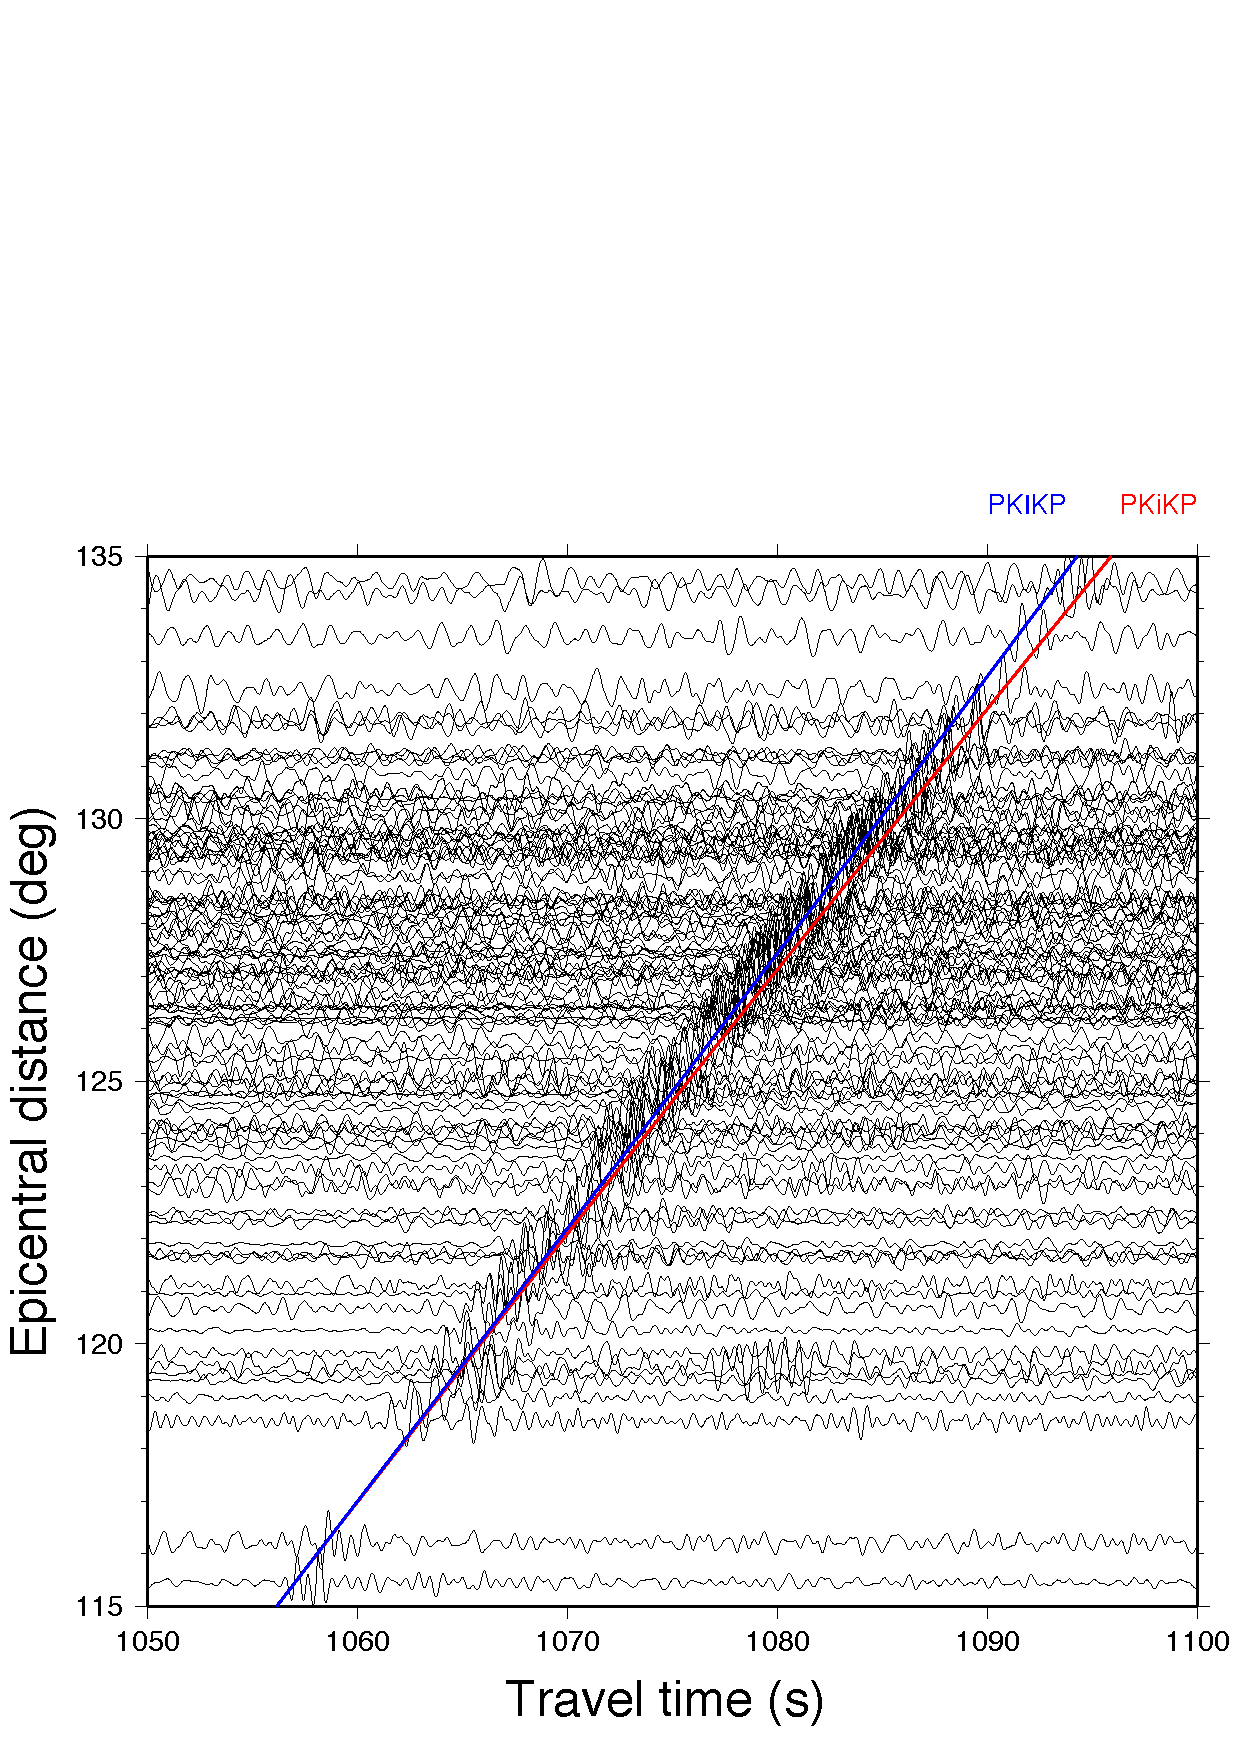
\includegraphics[width=0.6\textwidth]{figures/celebessea/celebessea_real.pdf}
	\caption{Real seismogram data from the Celebes Sea event after event selection. Each seismogram is zeroed on the earthquake time. Over plotted lines are theoretical phase arrivals computed using the AK135 model. Only data with a clear PKIKP arrival are plotted}
	\label{fig:Real nonaligned}
\end{figure}

\begin{figure}
	\centering
	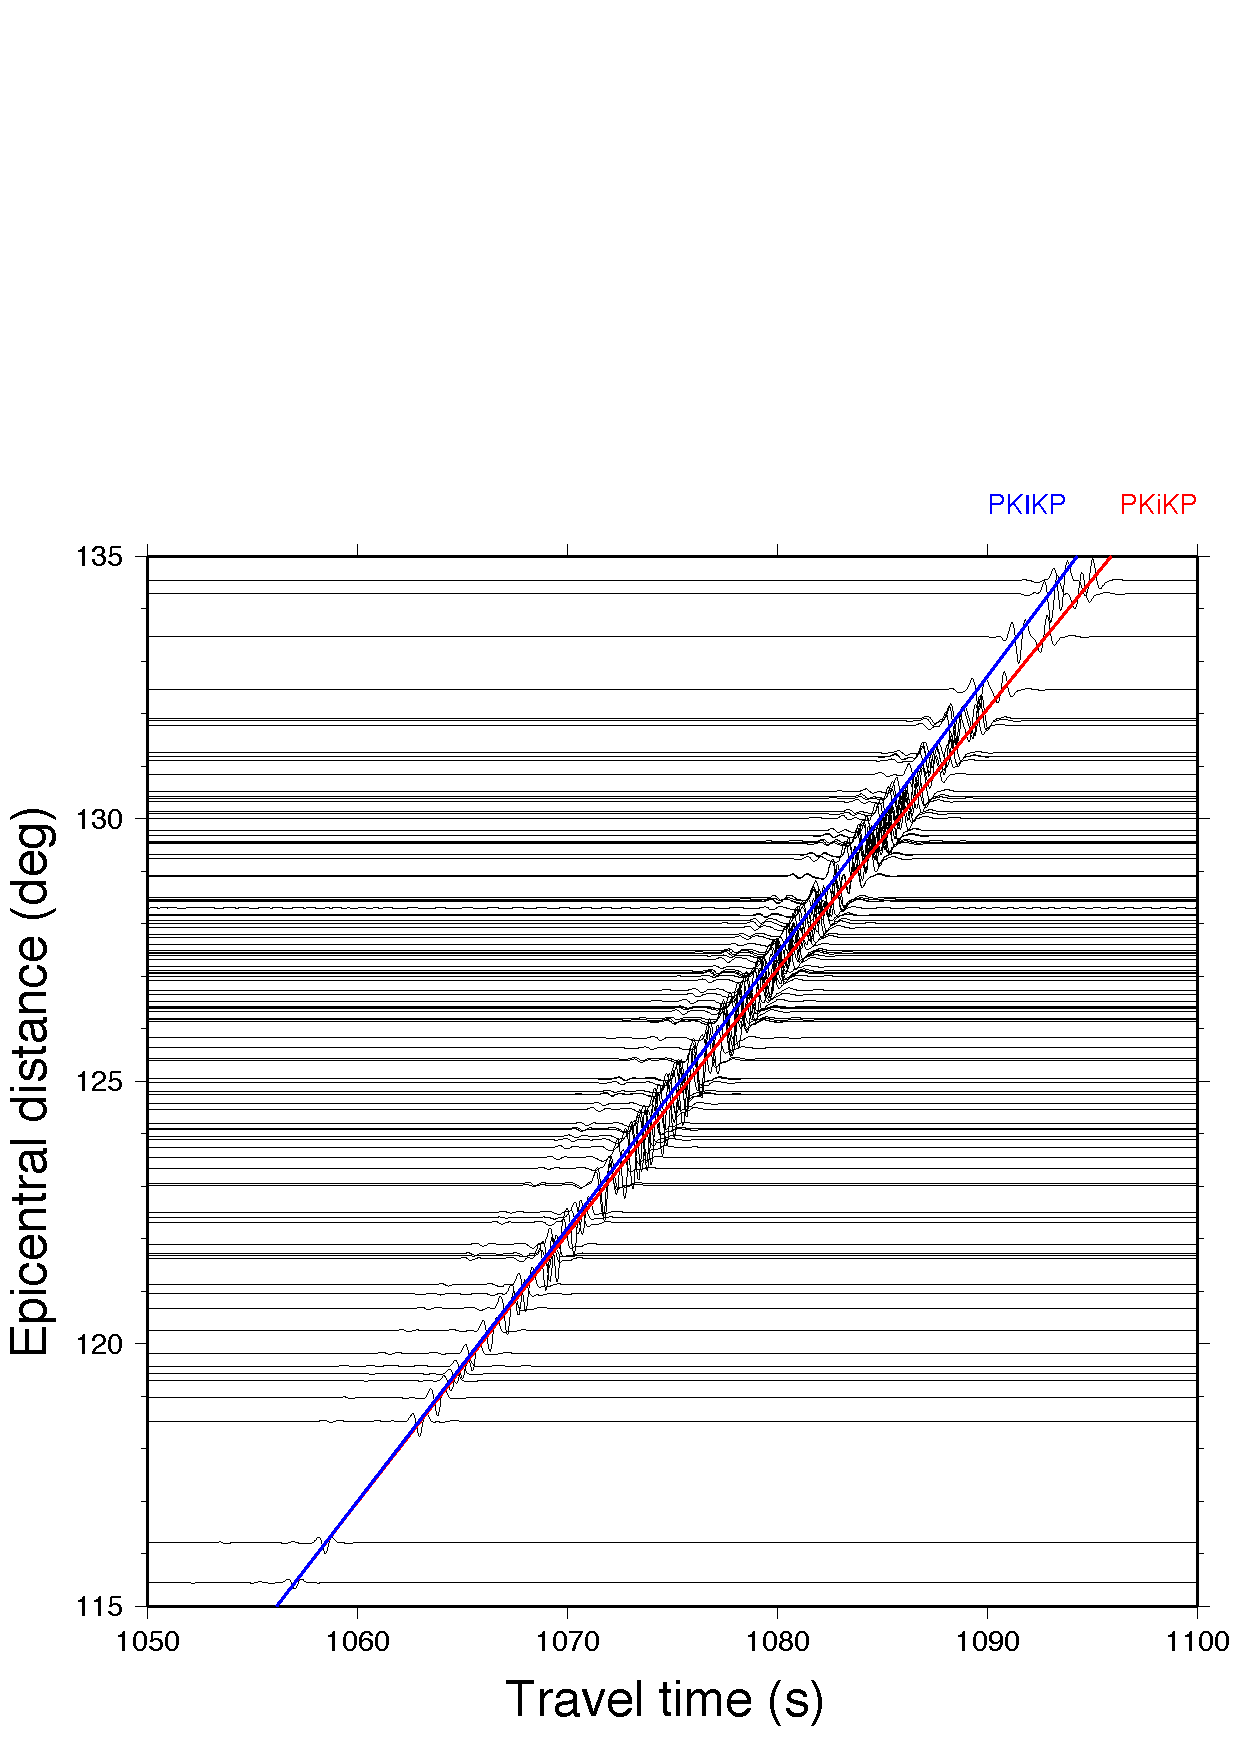
\includegraphics[width=0.6\textwidth]{figures/celebessea/celebessea_synthetic_both.pdf}
	\caption{Synthetic seismogram data for the Celebes Sea event.. Each seismogram is zeroed on the earthquake time. Over plotted lines show theoretical phase arrivals computed using the AK135 model.}
	\label{fig:Synth nonaligned}
\end{figure}

In order to more easily visualise the two phases we plot individual PKiKP, PKIKP and both combined synthetic seismograms. Each of these is shifted such that the final PKiKP upswing occurs at zero time. This is shown in figure \ref{fig:Synth aligned}. It is now clear to see the PKiKP phase merging with the PKIKP phase at low epicentral distances.

\subsection{Quantifying minimum resolvable difference}
The only two features that are measurable at all distances in the combined synthetic seismograms are the initial upswing and the final upswing (see figure \ref{fig:Synth aligned}). When making measurements of real data we want to be sure that we are measuring a PKIKP (initial upswing) and PKiKP (final upswing) feature, and not two PKiKP features. Measuring two PKiKP features is more likely at lower epicentral distances due to the PKIKP phase getting weaker, and the PKiKP phase developing a large upswing to the left. Incorrectly measuring two PKiKP features would cause a systematic overestimate of the true difference between the two phases. We also note that this is not a problem for synthetic data, where we can take measurements of the two phases individually.

\begin{figure}
	\centering
	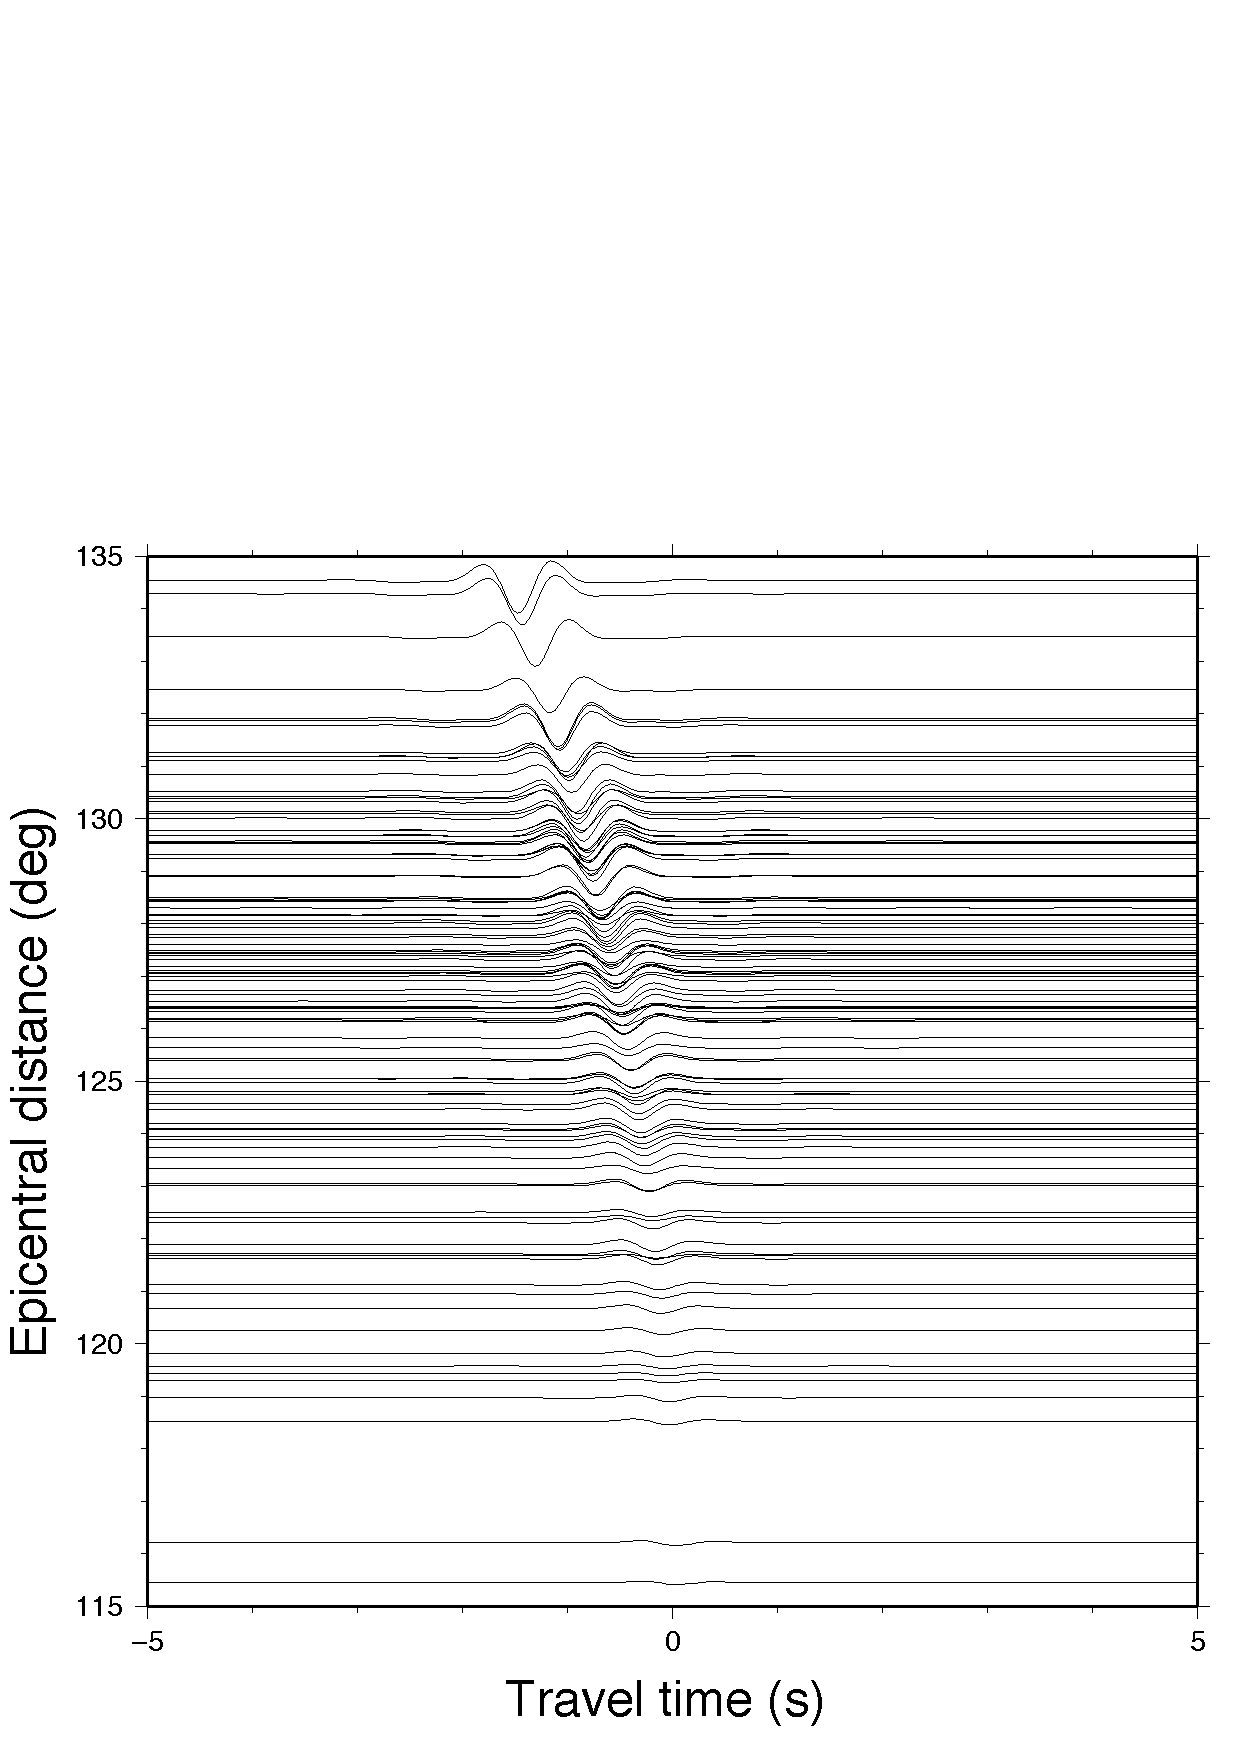
\includegraphics[width=0.4\textwidth]{figures/celebessea/celebessea_KIK_aligned}
	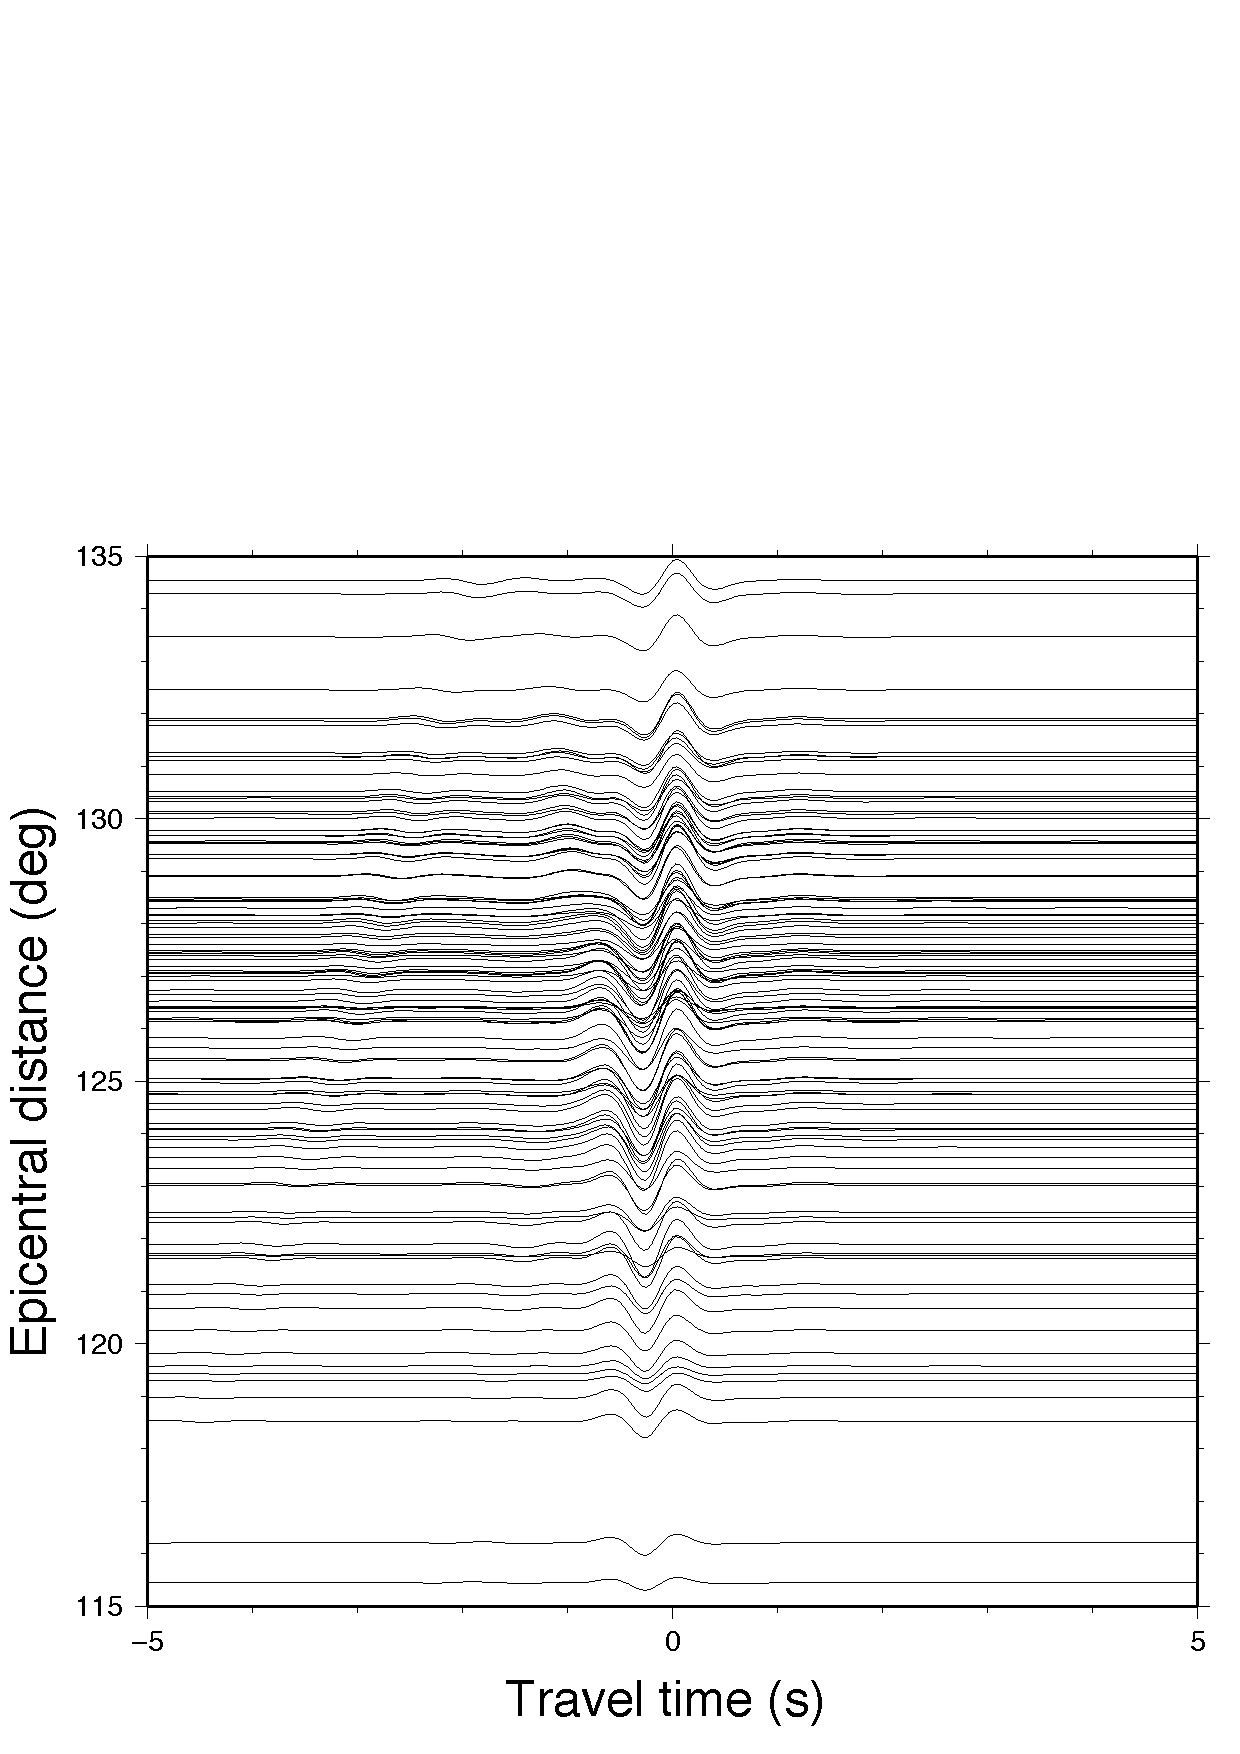
\includegraphics[width=0.4\textwidth]{figures/celebessea/celebessea_pkikp_aligned}
	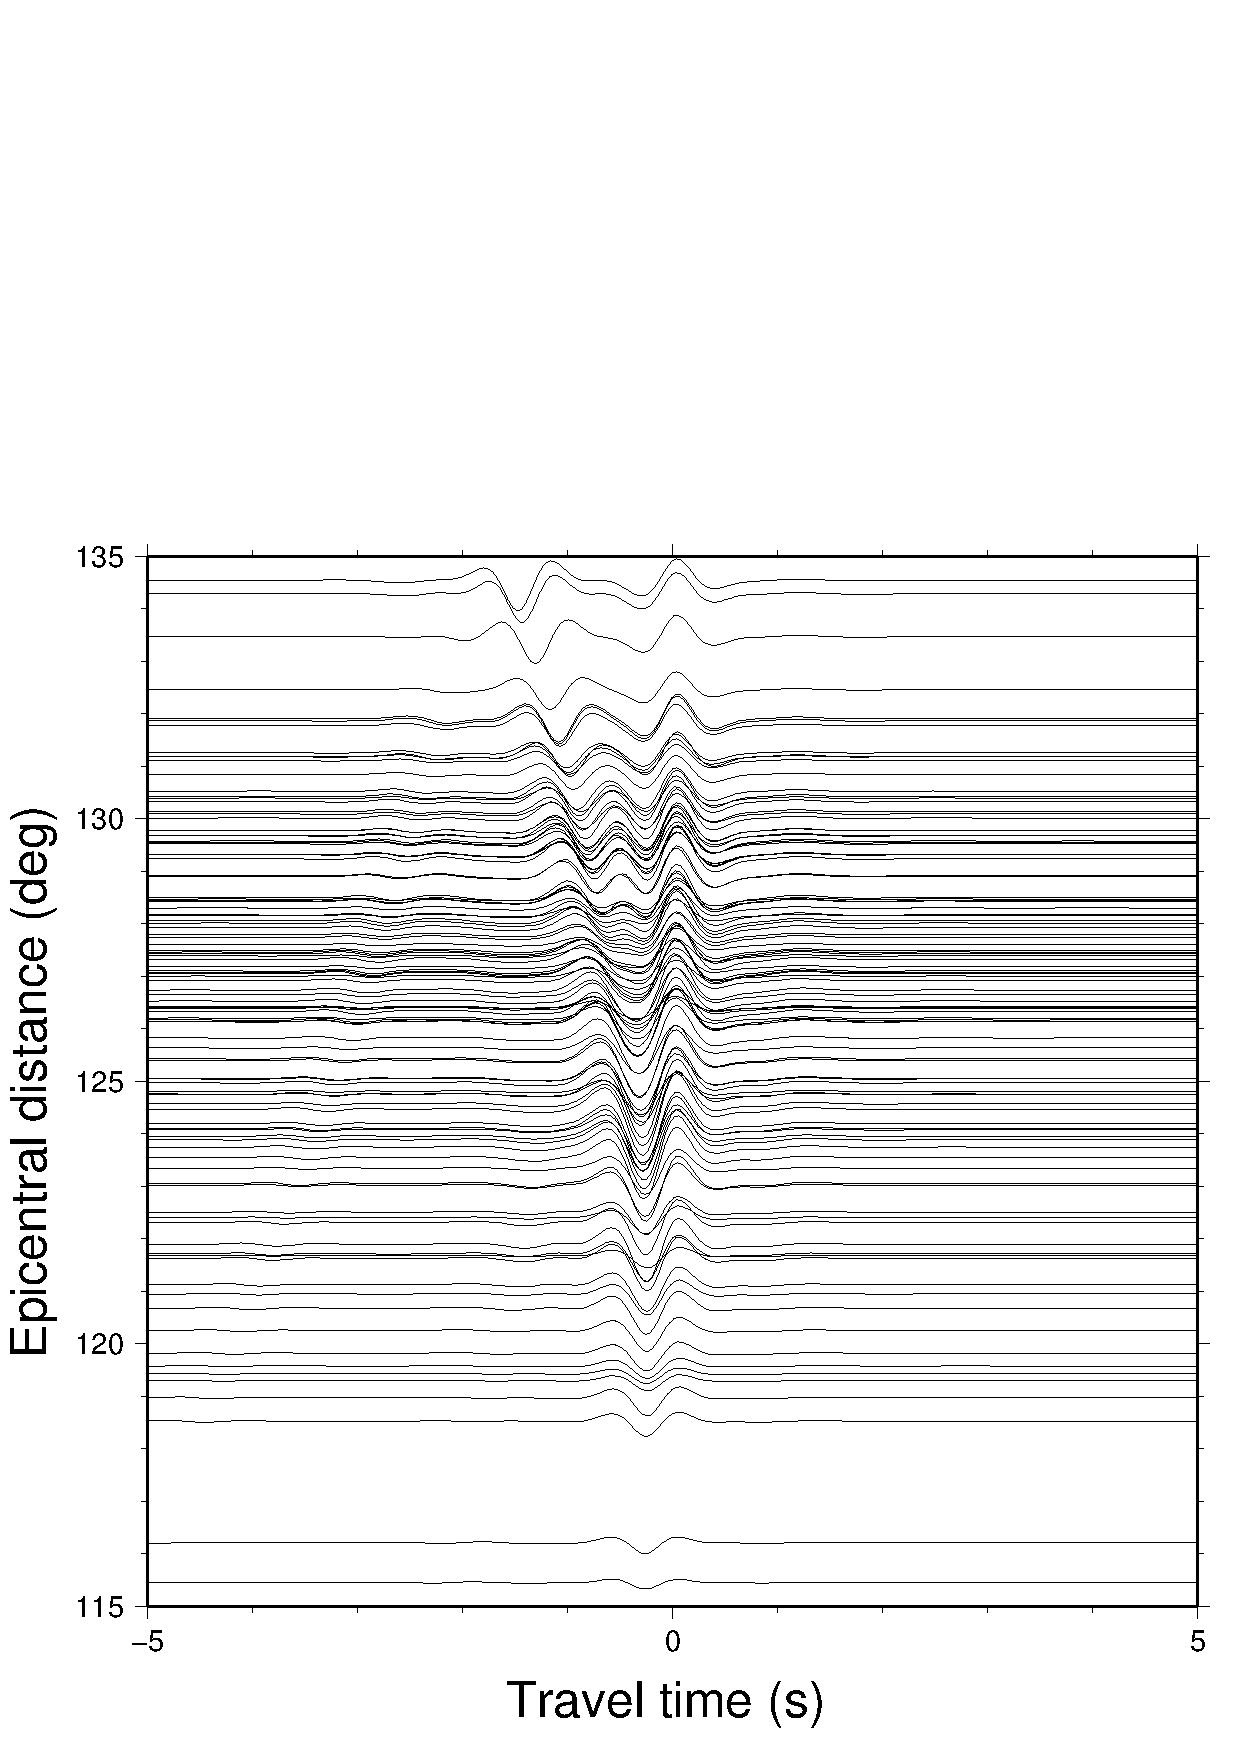
\includegraphics[width=0.4\textwidth]{figures/celebessea/celebessea_both_aligned}
	\caption{Separated PKIKP (top left) PKiKP (top right), and combined (bottom) synthetic seismograms for the Celebes Sea event.}
	\label{fig:Synth aligned}
\end{figure}

Small differences in the real and model velocity structures are expected only to affect the difference in arrival times between the two phases. We can therefore derive a minimum value ($t_{0}$) for $ \left ( t_{PKiKP} - t_{PKIKP} \right )_{observed}$, at and below which we should not trust measurements.

Figure \ref{fig:Min distance} shows measurements of peak to peak differences for PKiKP, PKIKP and combined synthetic waveforms computed for the Celebes Sea event. In each case the upswings furthest to the left and right are measured, and the difference taken between these two peaks. The three lines of best fit, fitted in the range $0.67s < t < 0.75s$, meet at $ t_{0} = 0.68s$. Below this difference the PKiKP and combined measurements coincide as expected, and it is impossible to measure an accurate difference on a combined seismogram.

\begin{figure}
	\centering
	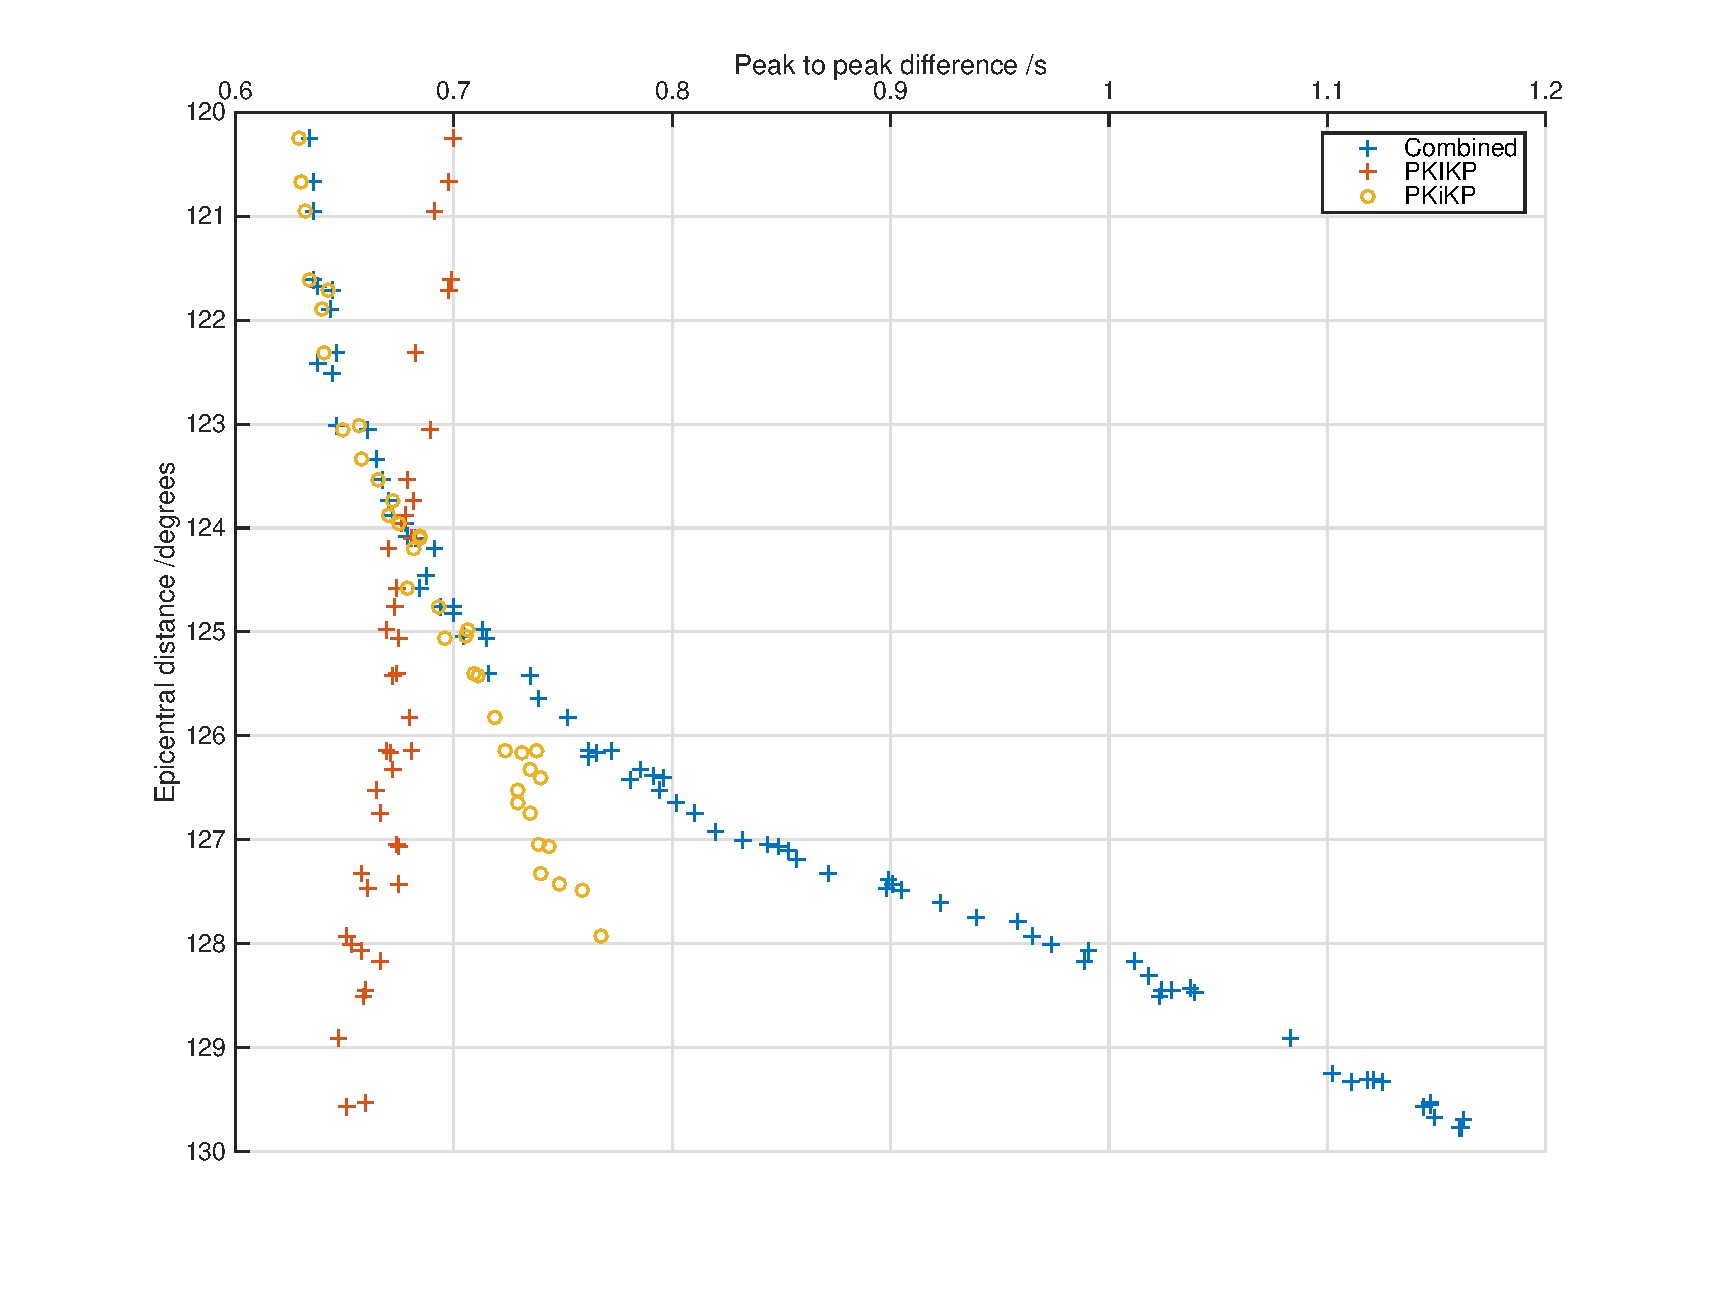
\includegraphics[width=0.8\textwidth]{figures/min_distance}
	\caption{Peak to peak travel times recorded from synthetic data shown in figure \ref{fig:Synth aligned}. Differences are measured between the leftmost and rightmost upswings. Data is shown for combined (blue), PKIKP (red) and PKiKP (yellow) seismograms. Lines of best fit are fitted using those values in the range $0.67s < t < 0.75s$.}
	\label{fig:Min distance}
\end{figure}

As a consequence all real data measurements must conform to
\begin{equation}
	\left ( t_{PKiKP} - t_{PKIKP} \right )_{observed} > t_{0}
\end{equation}
This in conjunction with equation \eqref{eq:Residual definition} gives an inequality that each individual residual must satisfy for it to be a reliable measurement
\begin{equation}
	\delta t > t_{0} -  \left ( t_{PKiKP} - t_{PKIKP} \right )_{model}
	\label{eq:Residual ineq}
\end{equation}
At deeper depths where $ \left ( t_{PKiKP} - t_{PKIKP} \right )_{model} $ is high we can therefore measure a large range of negative $\delta t$, whereas at shallower depths we are restricted to only being able to measure positive values of $\delta t$.

The above analysis explains the limitations of our method as applied to measured data, allowing us to instantly know whether to trust the data or not. Eventually we will be interested in the range of velocity perturbations that are measurable using this method. Substituting equation \eqref{eq:Residual ineq} into equation \eqref{eq:Delta v} gives a fundamental limit on the range $\delta v$ that is measurable using this experimental methodology
\begin{equation}
	\delta v >  \frac{t_{0} -  \left ( t_{PKiKP} - t_{PKIKP} \right )}{t} v
	\label{eq:Fundamental lim}
\end{equation}
where all quantities are those measured using the initial model.

In order to help visualise equation \eqref{eq:Fundamental lim} we plot $\delta v$ as a function of depth in figure PUT LIMIT FIGURE HERE.
\subsection{Residual travel time analysis}
Figure \ref{fig:Real aligned} shows algined real world data. The PKIKP (leftmost phase) is not moving in as epicentral distance increases here, immediately showing that large positive residuals are expected at low epicentral distances (and hence depths).

\begin{figure}
	\centering
	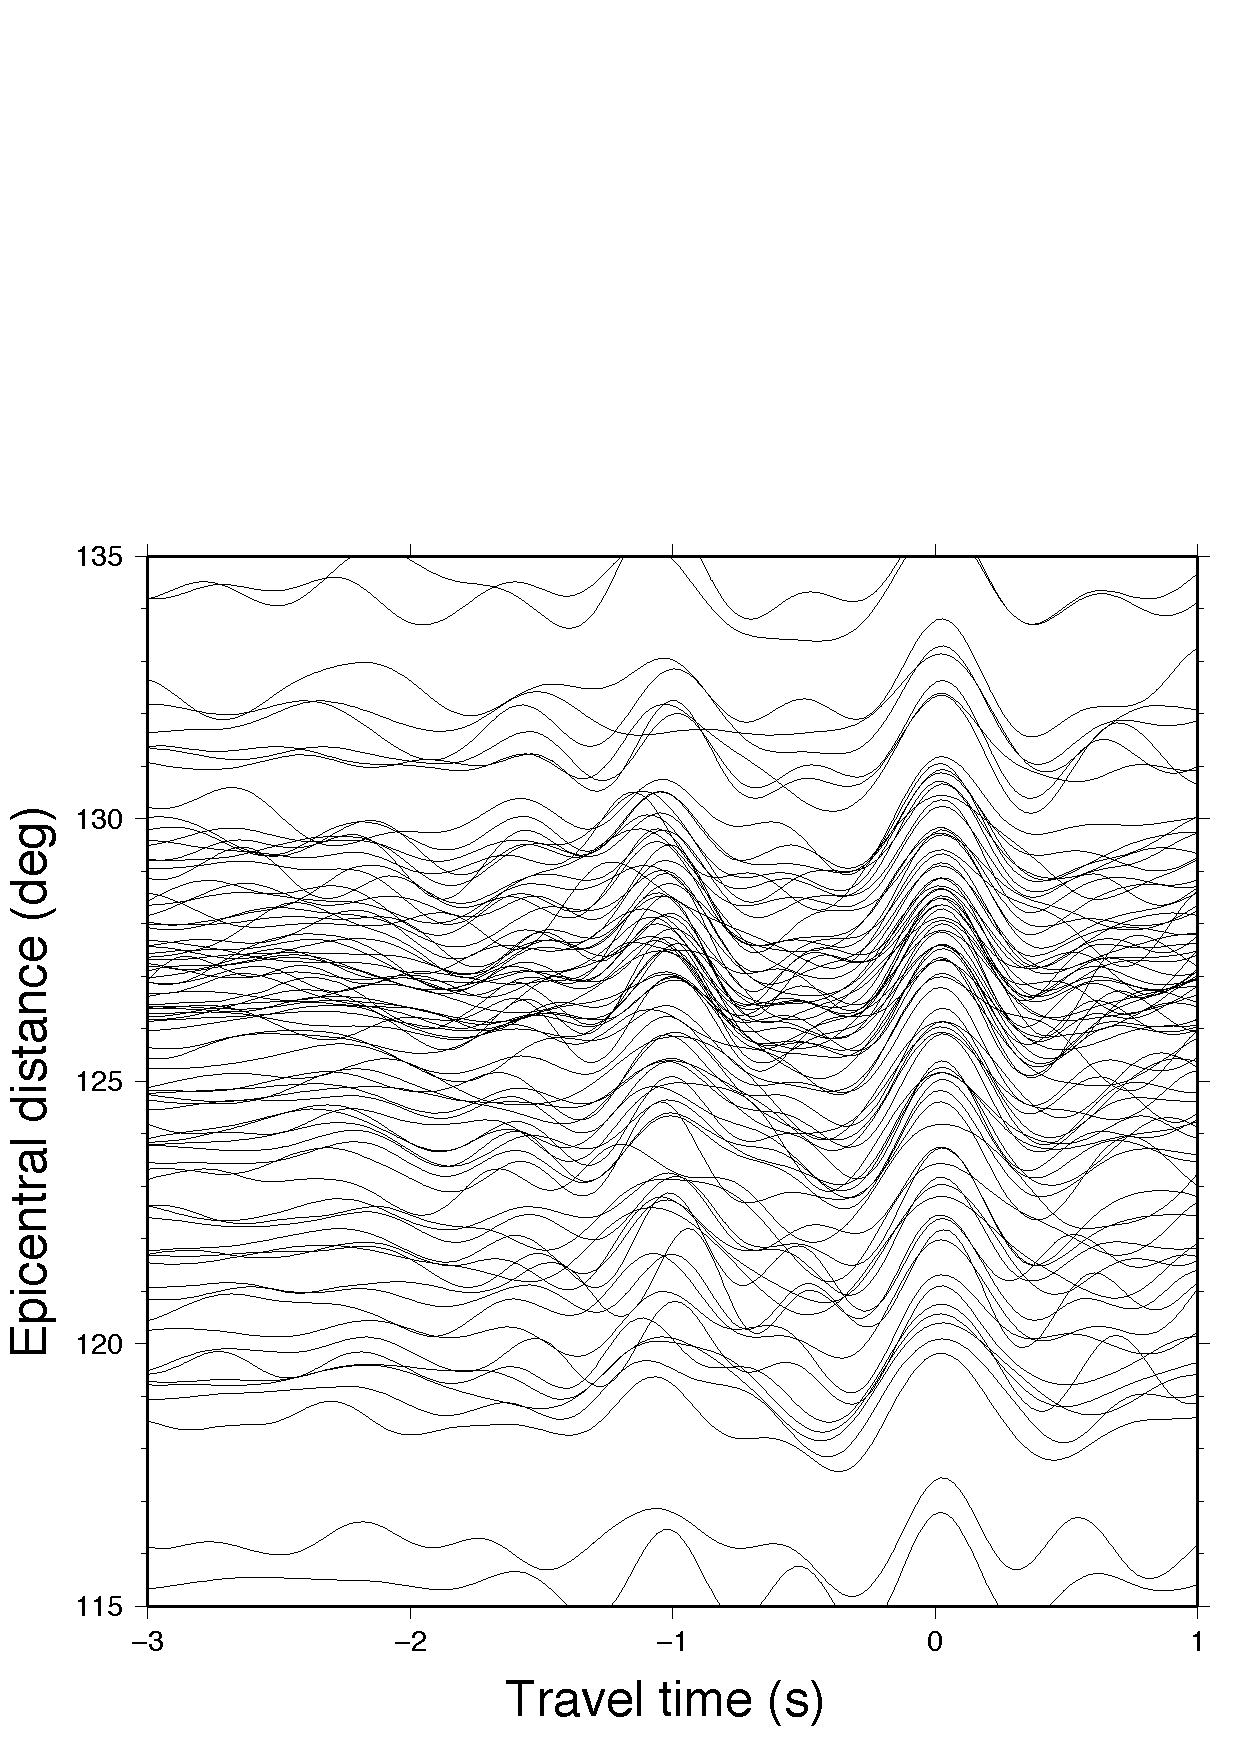
\includegraphics[width=0.6\textwidth]{figures/celebessea/celebessea_real_aligned.pdf}
	\caption{Real seismogram data for the Celebes Sea event. Each seismogram is zeroed on the final PKiKP upswing. Only data with clear PKIKP arrivals and clear PKiKP final upswings are plotted.}
	\label{fig:Real aligned}
\end{figure}

%%%%
\appendix
\section{Software details}
\label{app:Software}
The following lists the software used in this paper along with brief descriptions of what each piece of software was used for.
\begin{itemize}
	\item IRIS Wilber
	\begin{itemize}
		\item Used to select events and download worldwide seismic data from each selected event.
	\end{itemize}
	\item Centroid Moment Tensor (CMT) Catalogue
	\begin{itemize}
		\item Used to set earthquake time and location, and to feed WKBJ with resolved moment tensors on an event by event basis.
	\end{itemize}
\end{itemize}

%%%%
\newpage
% Bibliography
\bibliographystyle{yahapj}
\bibliography{/Users/dstansby/Physics/Papers/library}

\end{document}